\documentclass[11pt]{article}
\usepackage{amsmath, amssymb, amsthm}

\usepackage[pdftex]{graphicx}
\usepackage{tikz}
\usetikzlibrary{intersections}

\usepackage{marginnote}
\usepackage{endnotes}

\usepackage{fancyhdr}

%Listings stuff
\usepackage{listings}
\usepackage{lstautogobble}
\usepackage{color}

\definecolor{gray}{rgb}{0.5,0.5,0.5}
\lstset{
basicstyle={\small\ttfamily},
tabsize=3,
numbers=left,
numbersep=5pt,
numberstyle=\tiny\color{gray},
stepnumber=2,
breaklines=true
}

%Format stuff
\pagestyle{fancy}
\headheight 35pt

%Header info
\chead{\Large \textbf{Kosaraju's Two-Pass Algorithm}}
\lhead{}
\rhead{}

\begin{document}
\section{Algorithm}
	The strongly connected components (SCC's) of a directed graph $G$ are its maximal strongly connected subgraphs, where a strongly connected subgraph is one where there is a path from each vertex to every other vertex.
	
	\begin{lstlisting}[autogobble=true]
		def kosaraju(G):
			S = stack()
			G_rev = reverse(G)	#Reverse all the edges in G
			
			#Pass 1
			for v in G_rev:
				if v unexplored:
					explore(v)
					DFS_pass1(G_rev, v, S)
			
			#Pass 2
			while not empty(S):
				v = S.pop()
				if v explored:	#Flipped after pass 1
					unexplore(v)
					SCC rooted at S = DFS_pass2(G, v)
					
		def DFS_pass1(G, v, stack):
			for (v, w) in G:
				if w unexplored:
					explore(w)
					DFS_pass1(G, w)
			stack.push(v)
			
		def DFS_pass2(G, v):
			nodes = []
			for (v, w) in G:
				if w explored:
					unexplore(w)
					nodes += w
					DFS_pass2(G, w)
			return nodes
	\end{lstlisting}
	
	Essentially, the algorithm sorts the vertices in the graph by DFS ``finishing time'' and then iterates backwards through them to conduct one more DFS to uncover the SCC's. The second pass only explores ``sink'' nodes of a respective SCC.
	
\section{Analysis/Correctness}
	The SCC's of $G$ themselves introduce a ``meta-DAG'', in that if they are collapsed into nodes and the paths between then are maintained, the resulting graph is also a DAG.
	
	\subparagraph{Key Lemma} Consider 2 adjacent SCC's in $G$:
	
	\begin{center}
	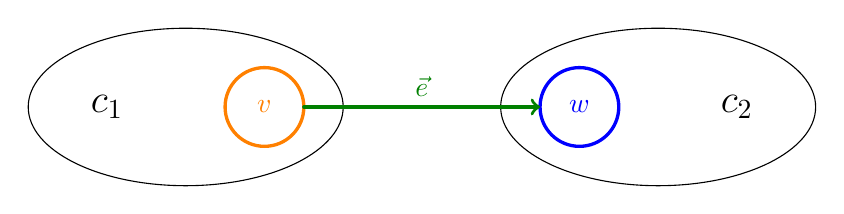
\begin{tikzpicture}
		[scale=1,line cap=round,
		%Styles
		axes/.style=,
		important line/.style={very thick},
		information text/.style={rounded corners,fill=red!10,inner sep=1ex},
		dot/.style={circle,inner sep=1pt,fill,label={#1},name=#1}			
		]
		
		%Colors
		\colorlet{anglecolor}{green!50!black}	%angle arcs/lines
		
		%The graphic
		\draw (0, 0) ellipse (2 and 1);
		\draw[color=orange, very thick] (1,0) circle (.5) node {$v$};
		
		\draw (6, 0) ellipse (2 and 1);
		\draw[color=blue, very thick] (5, 0) circle (.5) node {$w$};
		
		\draw[color=anglecolor, very thick,->] (1.5,0) -- node[above]{$\vec{e}$} (4.5,0);
		
		\node[font=\Large\bfseries] at (-1, 0) {$c_1$};
		\node[font=\Large\bfseries] at (7, 0) {$c_2$};
	\end{tikzpicture}
	\end{center}
	
	If $f(v)$ is the position on the stack of node $v$, with higher values corresponding to positions towards the top of the stack, then:
	\begin{equation}
		\max_{\substack{ \\ v \in c_1}} f(v) < \max_{\substack{ \\ w \in c_2}} f(w)
	\end{equation}
	
	\subparagraph{Proof of Key Lemma} In the first pass of the algorithm, all of $c_1$ is explored before $c_2$ because the meta-graph is acyclic. That is, if the first $v$ chosen in the looped DFS is inside $c_2$, the algorithm will trace paths all the way to a ``sink'' vertex in $c_1$ and push the rest of its nodes onto the stack before backtracking to $c_2$.
	
	\subparagraph{Corollary} From the key lemma, we deduce that the maximum f-value (top of the stack) must lie in the sink SCC in the meta-graph.
	
	\begin{center}
	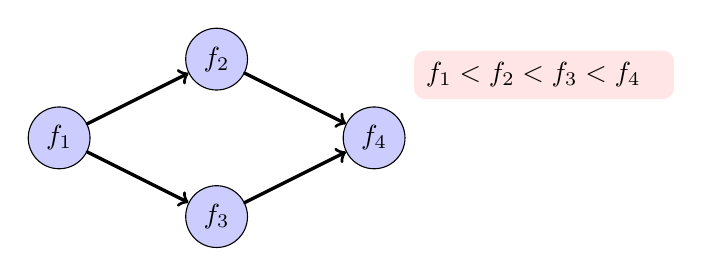
\begin{tikzpicture}
		[scale=1,line cap=round,
		%Styles
		axes/.style=,
		important line/.style={very thick},
		information text/.style={rounded corners,fill=red!10,inner sep=1ex},
		dot/.style={circle,inner sep=1pt,fill,label={#1},name=#1},
		main node/.style={circle,fill=blue!20,draw}			
		]
		
		%Colors
		\colorlet{anglecolor}{green!50!black}	%angle arcs/lines
		
		%The graphic
		\node[main node] (1) at (0, 0) {$f_1$};
		\node[main node] (3) at (2, -1) {$f_3$};
		\node[main node] (2) at (2, 1) {$f_2$};
		\node[main node] (4) at (4, 0) {$f_4$};
		
		\path[->, very thick]
			(1)	edge (3)
				edge (2)
			(2) edge (4)
			(3) edge (4);
			
		\draw[xshift=4.5cm](0,.8)
			node[right,text width=3cm,information text]
			{$f_1<f_2<f_3<f_4$};
	\end{tikzpicture}
	\end{center}
	
	\subparagraph{Correctness Intuition} By the above corollary, the second pass of the algorithm begins in a sink SCC, $c^*$. The first DFS uncovers $c^*$, and the rest recurses on $G-c^*$.
	
	\subparagraph{Runtime} Because the algorithm is really just 2 DFS loops, it runs in $O(m+n)$ time with some slow constants.

%	\begin{center}
%	\begin{tikzpicture}
%		[scale=3,line cap=round,
%		%Styles
%		axes/.style=,
%		important line/.style={very thick},
%		information text/.style={rounded corners,fill=red!10,inner sep=1ex},
%		dot/.style={circle,inner sep=1pt,fill,label={#1},name=#1}			
%		]
%		
%		%Colors
%		\colorlet{anglecolor}{green!50!black}	%angle arcs/lines
%		
%		%The graphic
%	\end{tikzpicture}
%	\end{center}

%	\begin{figure}[htb]
%		\centering
%		\includegraphics[width=0.8\textwidth]{filename.eps}
%		\caption{Caption.}
%		\label{fig:figure}
%	\end{figure}

%		\def\enotesize{\normalsize}
%		\theendnotes
\end{document}